\documentclass{thesisreport}
\usepackage{float}  %


\begin{document}
% Last modification: 2016-09-29 (Marc Deisenroth)
% Modification for UW: 2017-05-22 (jphickey)
\begin{titlepage}

\newcommand{\HRule}{\rule{\linewidth}{0.5mm}} % Defines a new command for the horizontal lines, change thickness here


%----------------------------------------------------------------------------------------
%	LOGO SECTION
%----------------------------------------------------------------------------------------



\begin{center} % Center remainder of the page

%----------------------------------------------------------------------------------------
%	HEADING SECTIONS
%----------------------------------------------------------------------------------------


\includegraphics[width = 6 cm]{./figures/ecn}\\[1.5cm] 
\textbf{\textsc{\Large Artificial Intelligence - ARTIN}}\\[1.0cm] 
\textsc{\Large École Centrale de Nantes}\\[0.5cm] 
%\textsc{\large CORO CSYS$^{1}$/ SUBJECT$^{2}$}\\[0.95cm] 

%----------------------------------------------------------------------------------------
%	TITLE SECTION
%----------------------------------------------------------------------------------------

\HRule \\[0.4cm]
{ \huge \bfseries SVM Laboratory Report}\\  % Title of your document
\HRule \\[1.5cm]
\end{center}
%----------------------------------------------------------------------------------------
%	AUTHOR SECTION
%----------------------------------------------------------------------------------------

%\begin{minipage}{0.4\hsize}
\begin{flushleft} \large
\textit{Authors:}\\
% Your name
LANCHA João\\
LOIZOU Ioannis\\
\end{flushleft}
\vspace{8cm}
\makeatletter
Date: November 29, 2023 

\vfill % Fill the rest of the page with whitespace



\makeatother


\end{titlepage}



 \include{thesisfront}  
 
  \section*{Abstract}
In this laboratory we are given the Caltech 101 dataset and a jupyter notebook with exercises and steps to follow. Goal of this activity is to perform binary classifications using different methods, first a linear classifier, and then support vector machines (SVMs). Later on, some performance measurements are calculated, and the results are compared between each method.
 \newpage
 \newpage
 \listoffigures
\listoftables
\tableofcontents
 


\chapter{Building the dataset}

 Caltech’s dataset consists of 10 folders containing a different number of images of a certain type of animal. Each folder is then a class. Since our goal is to perform binary classifications, we only need to take two classes, and also perform some pretreatment on the data.\\
For such task, we use a predefined function given in the notebook called \textit{“buildDataset”}, its inputs are:\\

\begin{itemize}
\item The directory where the images are stored. 
\item Names of the labels.
\item Maximum number of classes we want to keep for our dataset (K).
\item Maximum number of images to read from each folder (N).
\item Height/Width of the images in pixels. 
\item Random seed (to generate reproducible results).
\end{itemize}

In this exercise K = 2 and N = 100.  Meaning that we are going to have a dataset of two classes (this way we are able to do binary classification), with a maximum of 100 images per class. The height and width of the images are set to 100x100 pixels.\\
The function then selects two random categories of animals (classes), saves those names in a vector called \textit{“labelNames”}, goes through the images in these folders and reads them in greyscale and resizes them to the desired size. Next it flattens the matrix of grayscale values of each image to a vector and puts it in a matrix of two columns, one image per row. Therefore the first column contains the vector of grayscale values and the second column contains the label.\\

\begin{equation*}
\begin{bmatrix}
    \mathbf{v}_1 & 1 \\
    \mathbf{v}_2 & 0 \\
    \mathbf{v}_3 & 1 \\
    \mathbf\dots & \dots \\
    \mathbf{v}_n & 0 \\
    % Add more rows as needed
\end{bmatrix}
\quad \text{where} \quad
\begin{aligned}
    \mathbf{v}_n &= [x_{n1}, x_{n2}, x_{n3}, \dots, x_{n10000}] \\
\end{aligned}
\end{equation*}

\captionsetup{type=figure}
\captionsetup{justification=centering, labelsep=period}
\captionof{figure}{Matrix of images and label as well as vector with pixel values.}
\newpage

Next we need to split the data in the following fashion:

\begin{itemize}
    \item 80\% - Train set
    \item 20\% - Test set
\end{itemize}

For that we used scikit-learn's \textit{train\_test\_spli}t function

\newpage

\chapter{Support Vector Machines}
 \section{Linear Kernel}
The first exercise on the jupyter notebook consists in using a support vector machine model with a linear kernel in order to perform the binary classification. The procedure is as follows: 
\begin{itemize}
    \item Use scikit-learn's \textit{SVC()} function to declare the model.
    \item Train it using our training set.
    \item Test it (Make predictions on the test set).
    \item  Count the number of errors (FN + FP).
    \item Display the performance score (using \textit{SVM().score()}).
\end{itemize}
The obtained results are:
\begin{itemize}
    \item Score: \textit{0.7619}
    \item Errors: \textit{5}
\end{itemize}



It is important to highlight that when dealing with SVMs it is not necessary to normalize the features. As seen in the lectures, normalizing features will only affect the size of our hyperplane (meaning the hyperplane, in the case of a 2D example, a line, will be longer or shorter) but it does not affect the distance from each point to the hyperplane, which is what we are interested in, when dealing with SVMs.\\
We are then asked to make probabilistic predictions using this model, which seems to be irrelevant, since SVMs are inherently deterministic. However, there is a method to obtain probabilistic outputs from such model, called Patt scalling, or sigmoid calibration. This method consists in fitting a logistic regression model to the SVM decision values. This regression is then trained to map the SVM output to a probability.\\
With the probabilistic predictions, the performance score remained unchanged.

\subsection{Support Vectors}
The parameters of a linear SVM model are the coefficients describing the hyperplane. If the hyperplane is a line there are two parameters, the slope and the intercept.\\ % TO COMPLETE
Furthermore, linear kernel SVMs only have 1 hyperparameter, which is the regularization parameter (C). The purpose of this value is to control how many points are allowed to cross the SVM margin.\\
Therefore, increasing C tends to make our model more accurate, and at the same time, more prone to over-fitting, since the margin becomes smaller. On the other hand, decreasing C leads to less accuracy (more points are "allowed" to be misclassified), but also less prone to over-fitting.\\
In our exercise, we had 67 support vectors, which are the points at the margins. Below are some of them.\\
    \begin{figure}[htbp]
    \centering
    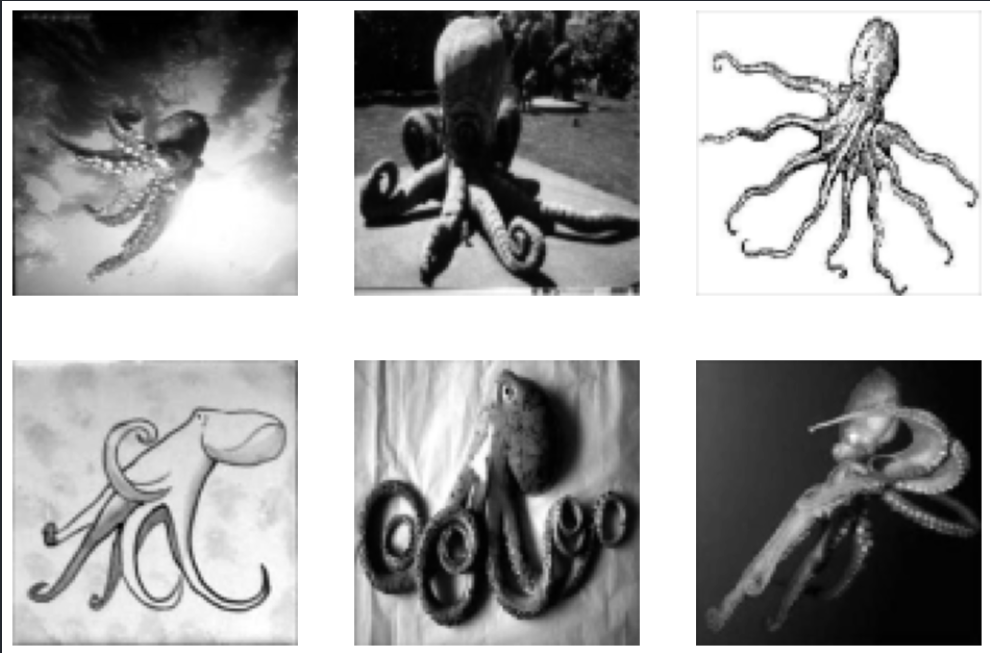
\includegraphics[scale=0.5]{./figures/supvecs}\\
    \caption{6 of the 67 support vectors.}
    \label{fig:bear 1000}
    \end{figure}

\newpage
 \section{Different Kernel SVMs}
 The following step consists in studying the impact of using different kernels in an SVM model. We repeated the procedure described in section 2.1 for 3 different kernels. It is important to highlight that each kernel presents different added hyperparameters, which affect the shape of the kernel. These are presented below.
 \begin{itemize}
    \item RBF - Radial Basis Function. (hyperparameters C, $\gamma$ -controls the width of the gaussian kernel)
    \item Sigmoid. (hyperparameters: C, $\alpha$ - scaling factor)
    \item Polynomial (Hyperparameters: C, degree of the polynomial)
\end{itemize}

The results obtained are presented in the table below: 
\begin{table}[H]
\centering
\begin{tabular}{|c|c|c|}
\hline
\textbf{Kernel} & \textbf{Support Vectors} & \textbf{Score} \\
\hline
\texttt{Linear} & 67 & 0.7619 \\
\texttt{rbf} & 79 & 0.6667 \\
\texttt{polynomial} & 72 & 0.7619 \\
\texttt{sigmoid} & 46 & 0.5238 \\
\hline
\end{tabular}
\caption{SVM Results}
\label{tab:svm-results}
\end{table}

\subsection{Hyper-parameter tuning}
As it was stated in the beginning of this section, introducing a different kernel to an SVM model adds the complexity of controlling the shape of this function. There will always be a kernel, and a given shape within that kernel, that will best classify the data, depending on the how our data points are distributed in the space. Therefore, in this step we do what is called a hyper-parameter tuning using scikit-learn's \textit{GridSearchCV()} function. It takes the model we previously declared and a hyper-parameter table as inputs. We do this step for each of the previous used kernels (linear, rbf, polynomial and sigmoid).\\
%Check ================================================================
The function gridSearchCV, which means Grid Search Cross-Validation, will, once \textit{GridSearchCV().fit()} is called, randomly split the given data set (in our case the training set) into two subsets. Subsequently, it proceeds to test all of the different hyper-parameter combinations, using one subset to fit the data, and the other to evaluate the performance score. It repeats this process 5 times, since we are using the default 5-fold cross validation. This way it can decide on the best hyper-parameter combination for that kernel.\\
It is important to highlight that, since the function is actively validating its choice of parameters, there is no need to split the data into train, test and validation sets.
%End Check ===========================================================
The hyper-parameter table contains a range of values for the hyper-parameters and can be seen in the table below:
\begin{table}[H]
\centering
\begin{tabular}{|c|c|}
\hline
    \textbf{Hyper-parameter} & \textbf{Values}\\
\hline
    \texttt{C} & 0.001, 0.01, 0.1, 1, 10, 1000 \\
    \texttt{$\gamma$} & 1, 0.1, 0.01, 0.001, 0.0001, 'scale' \\
    \texttt{degree} & 2, 3, 5, 7, 9 \\
\hline
\end{tabular}
\caption{Hyper-parameter table fed to \textit{GridSearchCV} for optimization.}
\label{tab:svm-hyperparameters}
\end{table}

The results obtained with \textit{GridSearchCV} are shown in the table below.

\begin{table}[H]
\centering
\begin{tabular}{|c|ccc|c|}
\hline
\textbf{Kernel} & \multicolumn{3}{c|}{\textbf{Hyperparameters}} & \textbf{Score} \\
\cline{2-4}
 & \textbf{C} & \textbf{$\gamma$} & \textbf{Degree} & \\

\hline
linear & 0.001 & 1 & 2 & 0.6667 \\
\hline
rbf & 10 & 0.001 & 2 & 0.8095 \\
\hline
poly & 0.01 & 0.01 & 2 & 0.7143 \\
\hline
sigmoid & 10 & 0.0001 & 2 & 0.6190 \\
\hline
\end{tabular}
\caption{SVM Kernel Results}
\label{tab:svm-kernel-results}
\end{table}


It is important to mention that, although not present in the hyper-parameter optimization table kernels can be seen as such, once they are in the borderline of creating a new method.\\
For some, having a  different kernel, means having a different model, for others, kernels are considered hyper parameters, as if they were a different tool that can be use to classify data, within an SVM model, once still, the underlying idea of optimal placement of the boundary is the same.
\newpage

\chapter{Performance Measures}
In this chapter we explore the different performance measures that can be used to indicate how good each model is, in classifying data. Firstly, we complete a predefined function to compute the confusion matrix and calculate some performance measures. Secondly, we move to other methods such as ROC curves, that are more suitable to compare different classifiers.
\section{Confusion Matrix}
In this section we were given a semi-completed function on the jupyter notebook, named \textit{compute\_measures}, which takes the lists of ground truth labels and predicted labels as inputs.\\
Inside the function we then start by building a confusion matrix, in other words, computing the amount of True positives, True negatives, False Positives and False negatives. For that, we go through a vector of two columns, with the first being the predicted label values, and the second being the ground truth labels, and we count the number of occurrences of a certain condition.\\
For true positives for example the condition is ground truth = prediction = 1, for true negatives is ground truth = prediction = 0.\\
Once the confusion matrix is built, we can then calculate measures such as accuracy, precision, specificity, recall, f-measure, negative predictive value and false predictive value.\\
Lastly, we compare these results with scikit-learn's \textit{classification\_report()}


\newpage

\section{ROC Curves}
ROC or Receiving Operating Characteristic curves are built for two purposes, getting the best threshold for a classifier, and comparing different classifiers. It plots false positive rate x true positive rate assuming a binary classifier returning the probability of an instance to belong to a class, and does that for all the different thresholds.\\
In the ideal case, our ROC curve would be a square with an area of 1 under its curve. On the other hand, a random classifier is a diagonal line that cuts this square in half. Therefore with an ROC curve we can already see if the classifier is predicting better than a random one.\\ 
Furthermore, since we want our classifier to have the highest number of true positives as possible, it has to be as close to the (0,1) point as possible in the ROC plot. However, when comparing classifiers, sometimes it is unclear which is closer. For that reason, the best metric to compare two different classifier.s is the area under the ROC curve. The higher it is, the better performing is the classifier.\\
It is important to highlight that this is a general rule, for some specific classifying tasks, such as checking weather a patient has a highly contaminating disease or not, we want a classifier that does not miss a single true positive, and that sometimes does not translate into having a bigger area under the curve as another classifier. Therefore, the comparison must be done without forgetting about the end goal of the task. 
%Check =========
In the following exercise, we are asked to plot the ROC curves for all SVM models with all the different kernels, before and after the hyper-parameter tuning. To do that we need probabilistic predictions using the method mentioned before. To be able to compare the different models, we need to compute the area under the curve which is called AUC. The area under the ROC curve clearly shows which is the most performant model in a classification task.
Firstly, we compare the models before the hyper-parameter tuning. The best performance is achieved from the SVM which has the rbf kernel, Followed by linear and poly with similar results and last with a big difference we have SVM with sigmoid kernel.\\
After the hyper-parameter tuning, rbf maintains the best performance with close second the linear. Poly improved but less compared to others. Notably the sigmoid became slightly worse. This can happen if the parameters defined before the tuning does not contain the initial hyper-parameters as well as due to the different selection of test and validation test.
Finally compared to a random classifier we can see that we have better results for all the models which means that the models are possibly useful.\\
Below is a table resuming all the ROC results, pre and post tuning.
\begin{table}[H]
\centering
\begin{tabular}{|c|c|c|}
\hline
\textbf{Kernel} & \multicolumn{2}{c|}{\textbf{Area under ROC curve}} \\
\cline{2-3}
 & \textbf{Pre-Optimization} & \textbf{Post-Optimization} \\
\hline
linear & 0.7685 & 0.8426 \\
rbf & 0.8333 & 0.8889 \\
poly & 0.7685 & 0.8148 \\
sigmoid & 0.6204 & 0.5926 \\
\hline
\end{tabular}
\caption{Area under ROC curves pre and post hyper-parameter tuning}
\label{tab:svm-scores}
\end{table}
\newpage


\begin{figure}[H]
    \centering
    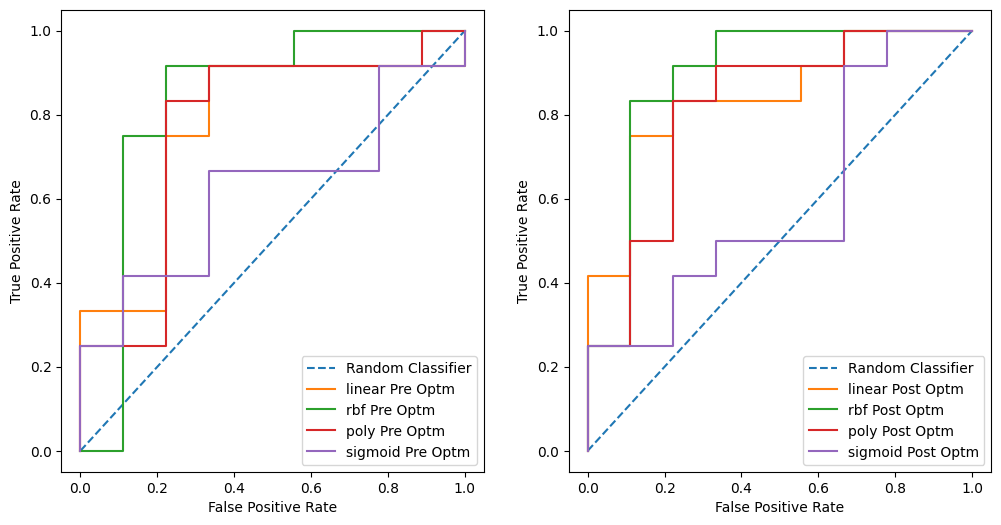
\includegraphics[width=1\linewidth]{figures/roc_curves.png}
    \caption{In the left ROC curves without tuning, In the right ROC curves with tuning}
    \label{fig:roc-before-after-tuning}
\end{figure}
\subsubsection{Logistic regression}
The results of the logistic regression are quite good especially when you compare them without the tuned hyper-parameters on the other models. The area under the curve is 0.8148.

\begin{figure}[H]
    \centering
    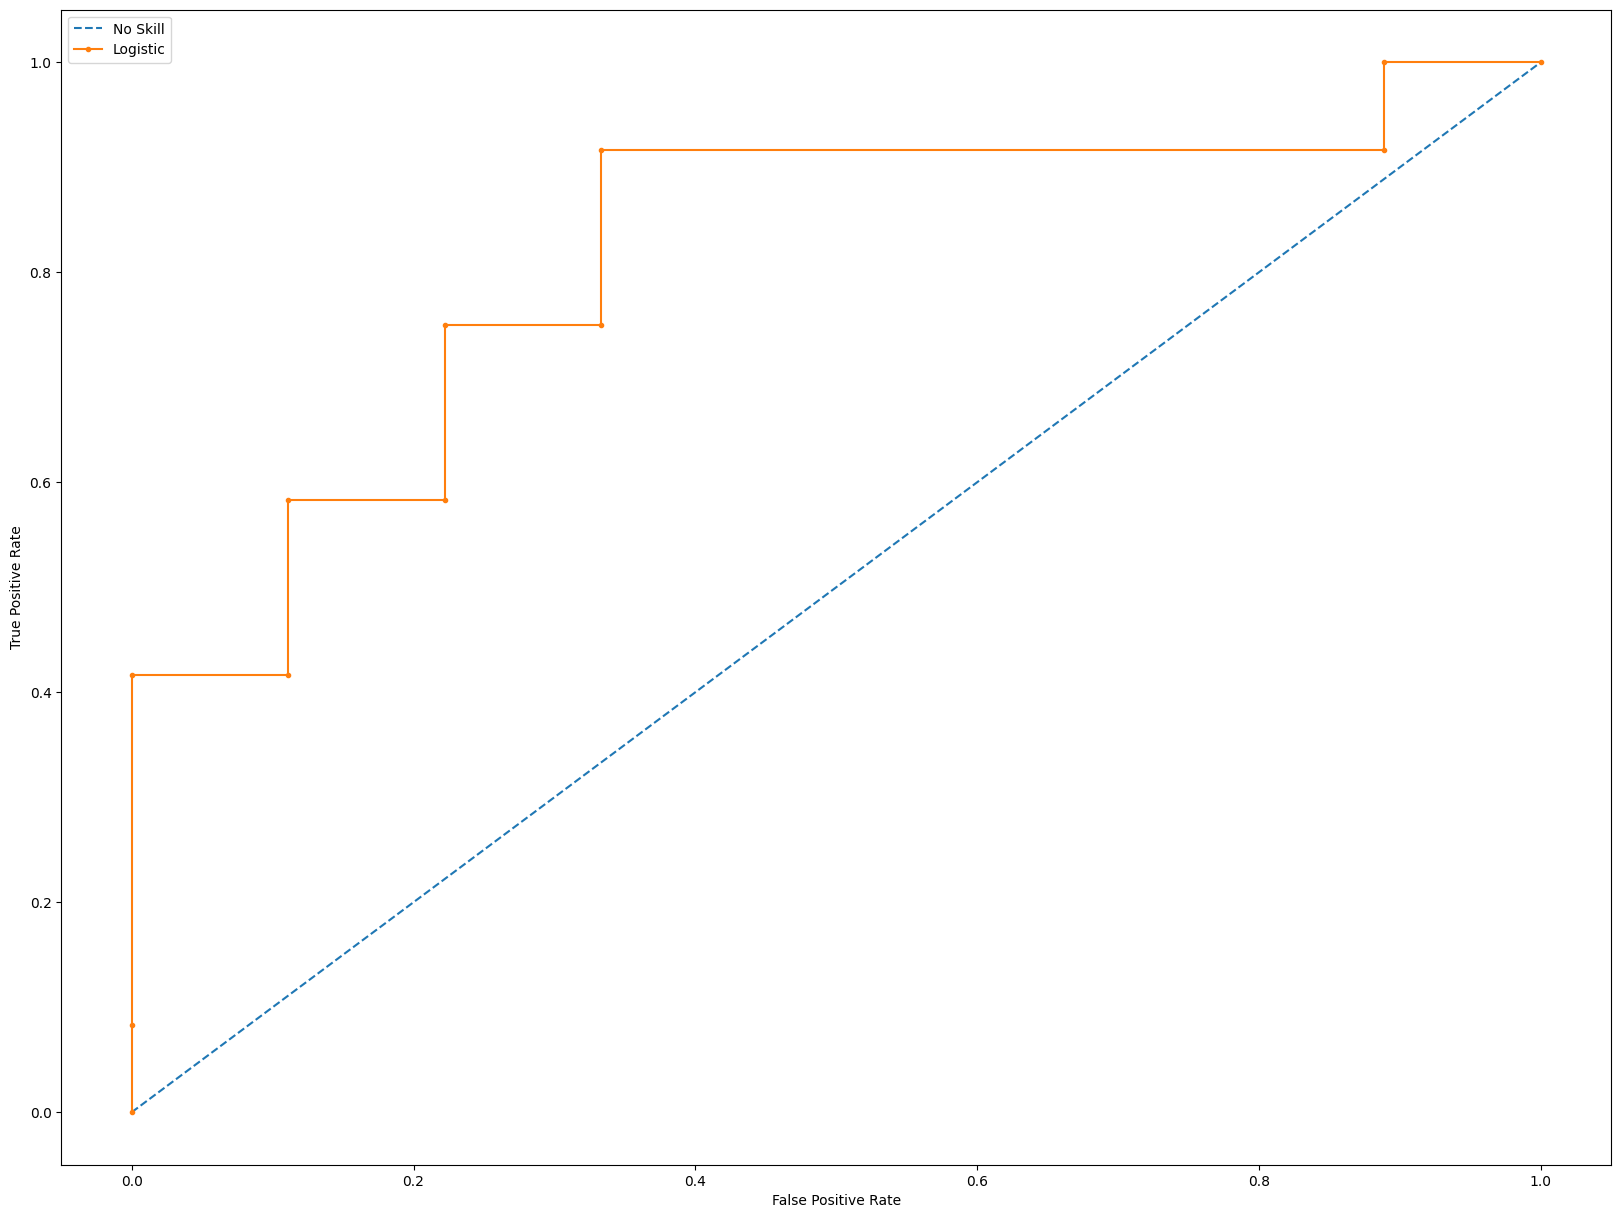
\includegraphics[width=0.7\linewidth]{figures/logistic_roc.png}
    \caption{ROC curve of logistic regression}
    \label{fig:roc-logistic}
\end{figure}

\section{Qualitative Results}

\begin{figure}[H]
    \centering
    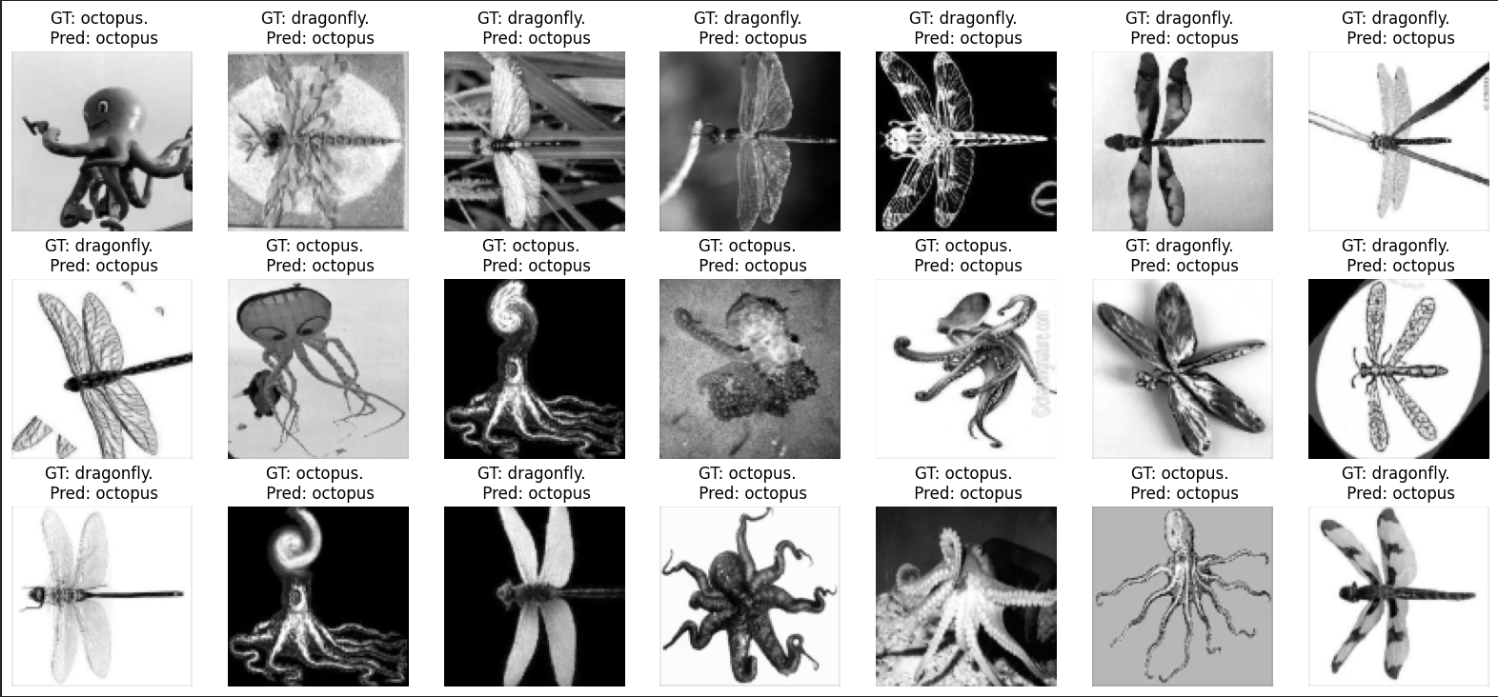
\includegraphics[width=1\linewidth]{figures/best_pred.png}
    \caption{Some predictions of our best model}
    \label{fig:best-pred}
\end{figure}

%End check ======== 
%Complete. 

 






    % \begin{figure}[htbp]
    % \centering
    % \includegraphics[scale=0.5]{./figures/yml file}\\
    % \caption{Declaration of a MDH table in a .yml file.}
    % \label{fig:bear 1000}
    % \end{figure}

    % \begin{figure}[H]
    % \centering
    % \includegraphics[scale=0.5]{./figures/jacobian}\\
    % \caption{Example of a jacobian matrix generated from a MDH table with the given code generator}
    % \label{fig:bear 1000}
    % \end{figure}
    % \begin{figure}[H]
    % \centering
    % \includegraphics[scale=0.5]{./figures/rvizsim}\\
    % \caption{Rviz simulation with control modes and estimated frame for a Kuka KR-16 robot}
    % \label{fig:bear 1000}
    % \end{figure}

\newpage

 \chapter*{Conclusion}
 \addcontentsline{toc}{chapter}{Conclusion}
 
 
In this project we showed how we can apply SVM for image classification and how to improve the results. As we showed hyper-parameter tuning is an important step which should not be neglected. Otherwise the model will not perform optimally.  
 
 
 \addcontentsline{toc}{chapter}{Bibliography}

 \begin{thebibliography}{9}
    \bibitem{mateus-lecture}
    Mateus, Diana.
    \emph{Artificial Intelligence}.
    Centrale Nantes, 2023.

    \bibitem{wiki-ai}
    Wikipedia.
    \url{https://en.wikipedia.org}.

    \bibitem{scikit-learn}
    scikit-learn.
    \url{https://scikit-learn.org}.
\end{thebibliography}
 
 
\end{document}